
\documentclass[border=8pt, multi, tikz]{standalone} 
\usepackage{import}
\subimport{../layers/}{init}
\usetikzlibrary{positioning}
\usetikzlibrary{3d} %for including external image 

\def\ConvColor{rgb:yellow,5;red,2.5;white,5}
\def\ConvReluColor{rgb:yellow,5;red,5;white,5}
\def\PoolColor{rgb:red,1;black,0.3}
\def\UnpoolColor{rgb:blue,2;green,1;black,0.3}
\def\FcColor{rgb:black,0.5;black,0.3}
\def\FcReluColor{rgb:blue,5;red,5;white,4}
\def\SoftmaxColor{rgb:magenta,5;black,7}   
\def\SumColor{rgb:blue,5;green,15}

\newcommand{\copymidarrow}{\tikz \draw[-Stealth,line width=0.8mm,draw={rgb:blue,4;red,1;green,1;black,3}] (-0.3,0) -- ++(0.3,0);}

\begin{document}
\begin{tikzpicture}
\tikzstyle{connection}=[ultra thick,every node/.style={sloped,allow upside down},draw=\edgecolor,opacity=0.7]
\tikzstyle{copyconnection}=[ultra thick,every node/.style={sloped,allow upside down},draw={rgb:blue,4;red,1;green,1;black,3},opacity=0.7]


\node (input) [opacity=1][canvas is zy plane at x=0] at (-8,0,0) {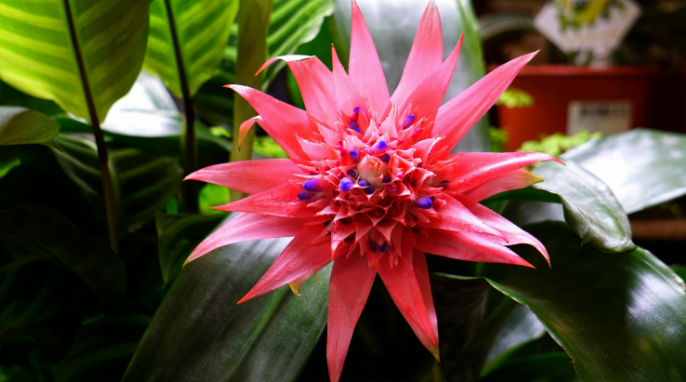
\includegraphics[width=2cm,height=2cm]{image_clef.png}};

\pic[shift={(-8, 0, 0)}] at (0, 0, 0) {Box={
    name=image,
    caption=,
    fill=white,
    opacity=0.0,
    height=0,
    width=0,
    depth=0
    }
};

\pic[shift={ (-5,0,0) }] at (0,0,0) 
    {RightBandedBox={
        name=ccr_b1,
        caption=\scriptsize Vision Transformer,
        fill=\ConvColor,
        bandfill=\ConvColor,
        height=30,
        width={ 12 , 12 },
        depth=30
        }
    };

\draw [connection]  (image-east)    -- node {\midarrow} (ccr_b1-west);

\pic[shift={ (3,0,0) }] at (ccr_b1-east) 
    {RightBandedBox={
        name=ccr_b2,
        caption=\scriptsize Quantum Layer (Boson Sampler),
        fill=\FcColor,
        bandfill=\FcColor,
        height=12,
        width={ 20 , 0 },
        depth=12
        }
    };

\draw [connection]  (ccr_b1-east)    -- node {\midarrow} (ccr_b2-west);

\pic[shift={ (2,0,0) }] at (ccr_b2-east) 
    {RightBandedBox={
        name=ccr_b3,
        caption=\scriptsize Linear Layer,
        fill=\ConvReluColor,
        bandfill=\ConvReluColor,
        height=12,
        width={ 3 , 0 },
        depth=12
        }
    };

\draw [connection]  (ccr_b2-east)    -- node {\midarrow} (ccr_b3-west);

\pic[shift={(2, 0, 0)}] at (ccr_b3-east) {Box={
    name=output,
    caption=\scriptsize Prediction,
    fill=red!20,
    height=1,
    width=1,
    depth=1
    }
};

\end{tikzpicture}
\end{document}
